\section{Direct reinforcement learning for combat}
The preceding studies optimized a myopic command-window objective. A separately frozen follow-up instead asks whether established PPO or DQN can improve actual combat outcomes \citep{schulman2017ppo,mnih2015human}. We use Stable Baselines3 2.9.0 \citep{raffin2021stable}, with newly collected game experience rather than the previous supervised labels. This is an algorithm screen, not a matched-data comparison against the older outcome models.

\paragraph{Frozen design.}
Protocol \texttt{d14a0b4} compares PPO with current observations, PPO with causal history and vanilla DQN with the same history. Three model seeds per family each receive exactly 32,768 Center interactions, totaling 294,912. All agents select fire/wait with the original rule steering and hard ammo/directive constraints. The 18-dimensional input contains seven normalized current-state features, ten history features or zeros, and remaining horizon. PPO variants have identical parameter counts but different information and effective capacity. Their two-hidden-layer, 64-unit networks have 10,947 actor/value parameters. DQN's online and target networks total 11,012 parameters. Optimization compute and behavior trajectories are not matched by equal interaction counts.

Reward is kill-count increase minus one on death minus 0.01 per issued-fire window. Both engine termination and the explicitly observed 180-window horizon terminate value bootstrap; this is a finite-horizon task, not an unobserved artificial timeout. Every window remains seven tics. There is no checkpoint or best-training-seed selection. Development compares all final fits on 24 new seeds per scenario. Eligible families need at least 0.5 additional Center kills, no more than 0.5 lost Line kills, and no more than 0.5 seconds shorter duration in either scenario, relative to event-memory rules. The family with the greatest Center kill gain receives one confirmation on 96 new seeds per scenario.

Confirmation retains all three fits and the current-only PPO reference, plus rules and event-memory rules. Against the event-memory rule, the primary gate requires at least one additional mean Center kill with a positive lower interval endpoint; Line kill and both duration lower endpoints must exceed $-1$ kill or second, respectively. Four contrasts use 20,000 paired crossed-bootstrap draws over game seeds and the three training fits, with 98.75\% intervals. Each episode's p95 decision time must be below 1 ms. These small-replicate intervals remain exploratory. Old command utility is secondary, and previous failed gates remain unchanged.

\paragraph{Development.}
History-PPO qualified with 3.278 additional Center kills and 4.292 additional Line kills over event-memory rules. Current-only PPO also qualified. DQN improved Center but lost 5.194 Line kills on average; its three Line fits averaged 30.50, 3.63 and 28.92 kills. This instability is specific to the tested data and budget, not a general algorithm ranking. PPO sacrificed the old command-efficiency utility by issuing more commands.

\paragraph{Simple-control addendum.}
While training was running, before development evaluations, we separately froze always-fire, alternating fire/wait and visible-target firing controls at \texttt{6a48cf8}. They preserve steering and hard constraints and cannot change the main selection or gate. On development seeds, history-PPO averaged 10.278 Center kills versus 8.000 for always-fire. On Line, both averaged 30.500, and every one of 10,728 compared PPO actions matched always-fire. No learned memory mechanism is needed to explain that Line result.

The diagnostic also demonstrates a measurement limitation. Always-fire and alternating fire/wait had identical kills, duration, engine reward and ammo use in all 48 paired development episodes. Yet all 1,319 hit windows for the alternating policy occurred during wait commands, so the old issued-fire-window utility credited none. Earlier values remain valid for their explicitly stated command-window estimand; they are not reliable combat-performance comparisons across arbitrary action schedules. The RL study chose kills as its primary endpoint before this diagnostic.

\paragraph{Fresh confirmation.}
The fixed history-PPO family passed the predeclared combat gate in 1,536 evaluation episodes. It averaged 11.559 Center kills versus 6.375 for event-memory rules, a difference of 5.184 ($[3.889,6.573]$). Center duration increased by 6.703 seconds ($[4.703,8.813]$). On Line, mean kills were 28.083 versus 25.365, a difference of 2.719 ($[1.073,4.417]$); duration changed by 1.428 seconds ($[-0.213,3.080]$), clearing the noninferiority boundary but not establishing longer duration. Maximum selected-model episode p95 decision times were 0.576 and 0.524 ms; both screens passed. Light reporting ran concurrently, so this is not a controlled systems timing result.

Against current-only PPO, history-PPO gained 2.188 Center kills ($[0.521,4.063]$) and 2.345 seconds ($[0.117,4.906]$) in exploratory secondary comparisons. Line's kill difference was 0.076 ($[-0.219,0.583]$). A general history advantage across scenarios is not established. The old net command utility declined by 0.738 in Center ($[-2.087,0.767]$) and 10.760 in Line ($[-12.943,-8.636]$) against event-memory rules. The new combat gate does not retroactively pass the old utility gates.


\paragraph{Fresh simple-control check.}
A further 576 control episodes used the confirmation seeds. History-PPO gained 3.017 Center kills over always-fire ($[2.024,4.115]$) and 4.403 over visible-target fire ($[3.292,5.542]$), in exploratory secondary comparisons outside the primary correction family. However, all 288 Line history-PPO episodes matched always-fire's issued-action sequence exactly. The Line advantage over event-memory rules therefore does not require a learned mechanism. Always-fire and alternating-fire again matched combat outcomes, while all 4,865 alternating-policy hit windows occurred during wait commands and went uncredited by the old utility.

\begin{figure}[H]
\centering
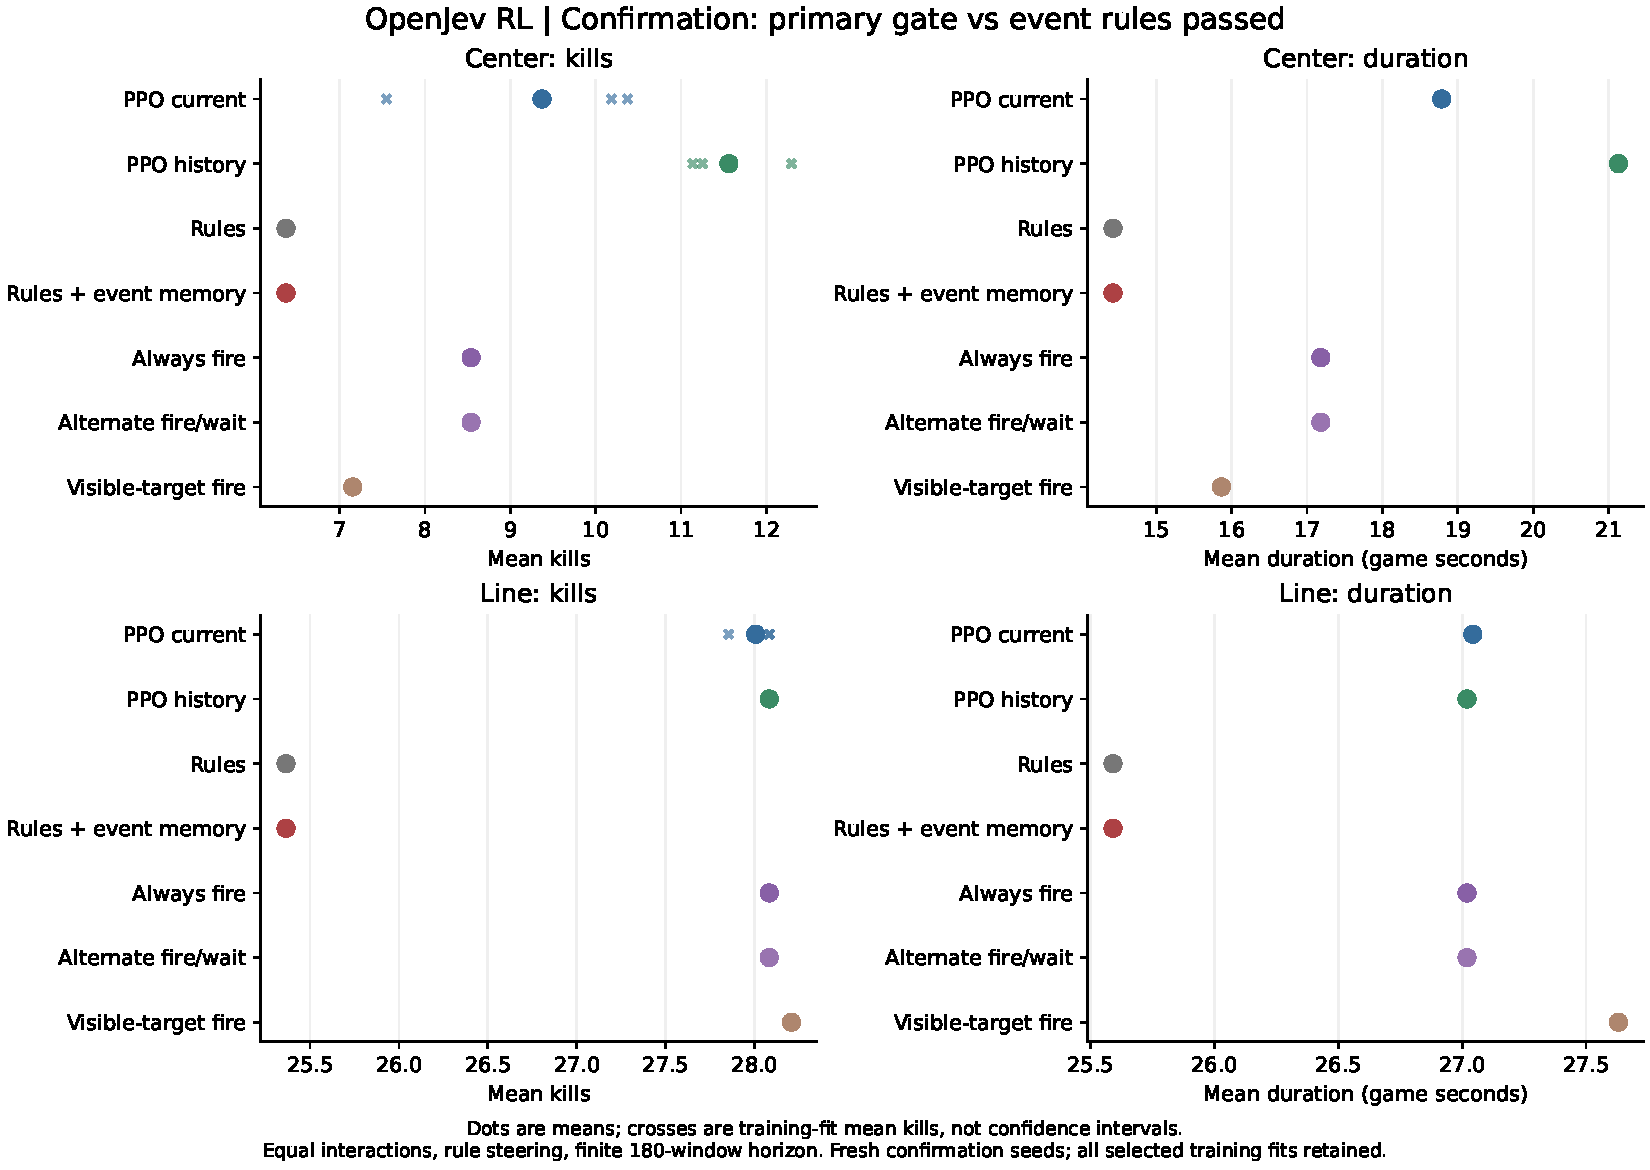
\includegraphics[width=\linewidth]{../evidence/rl-doom-v1/confirmation-results.pdf}
\caption{Fresh combat confirmation with the separately registered simple controls. Dots are means; crosses are training-fit mean kills, not confidence intervals. The primary gate compares history-PPO with event-memory rules. Simple-control comparisons constrain the interpretation of that pass.}
\end{figure}

The supported result is a useful Center firing controller, with positive secondary comparisons against current-only PPO and the tested simple patterns. It is not a new RL algorithm, a reproduction of proprietary RLCD, or a general recurrent-memory result. Only three training seeds and two scenarios were studied; both scenarios appeared in development. A stronger mechanism study would vary action timing or weapon delay, retain simple cadence controls, and test a second environment under a new prospective protocol.
